\documentclass[10pt,twopage]{acmsiggraph}

\usepackage{fancyheadings} % we need page numbers...
\usepackage{times}
\usepackage{graphicx}
\usepackage{hyperref}
\usepackage{latexsym}
\usepackage{hyperref}
\usepackage{amsmath}
\usepackage{amssymb}
\usepackage{amsthm}
\usepackage{amsfonts}
\usepackage{epsfig}


% allow for many figures and tables on one page
\renewcommand{\topfraction}{1.0} % all floats ok
\setcounter{totalnumber}{10}     % #floats = 10
\renewcommand{\textfraction}{0.0} % no text ok
\renewcommand{\dbltopfraction}{0.4}


% override page numbering conventions of the acm style
\pagestyle{fancyplain}
\lhead[\name]{}		% author name on the left for even pages
\rhead[]{\name}		% and on the right for odd pages
\setcounter{page}{1}	% I need to change this line for the proceedings


%%%%%%%%%%%
%
% Do not change anything above this line!!!
%
%%%%%%%%%%%



\begin{document}
\newcommand\result{0.01\%}
\newcommand\iteration{50000}

%%%%%%%%%%%%%%%%%%%%%%%%%%%%%%%%%%%%%%%%%%%%%%%%%%%%%%%%%%%%%%%%%%%%%%%%
%%%%%%%%%%%%%%%%%%%%%%%%%%%%%%%%%%%%%%%%%%%%%%%%%%%%%%%%%%%%%%%%%%%%%%%%
%
% Title and author(s)
%
%%%%%%%%%%%%%%%%%%%%%%%%%%%%%%%%%%%%%%%%%%%%%%%%%%%%%%%%%%%%%%%%%%%%%%%%
%%%%%%%%%%%%%%%%%%%%%%%%%%%%%%%%%%%%%%%%%%%%%%%%%%%%%%%%%%%%%%%%%%%%%%%%

\title{Poisson Image Solver}

\newcommand\name{C. Albert Thompson}

\author{\name\\
\\
Department of Computer Science\\
The University of British Columbia}

\maketitle

%%%%%%%%%%%%%%%%%%%%%%%%%%%%%%%%%%%%%%%%%%%%%%%%%%%%%%%%%%%%%%%%%%%%%%%%
%%%%%%%%%%%%%%%%%%%%%%%%%%%%%%%%%%%%%%%%%%%%%%%%%%%%%%%%%%%%%%%%%%%%%%%%
%
% Abstract
%
%%%%%%%%%%%%%%%%%%%%%%%%%%%%%%%%%%%%%%%%%%%%%%%%%%%%%%%%%%%%%%%%%%%%%%%%
%%%%%%%%%%%%%%%%%%%%%%%%%%%%%%%%%%%%%%%%%%%%%%%%%%%%%%%%%%%%%%%%%%%%%%%%

\begin{abstract}
For this paper we present a way to solve Poisson's equation and regenerate images from the divergence of the original image. We first looked at recent work that implement Poisson solvers. From that we found the steps need to decompose an image and find the divergence. Once we found the divergence we used Jacobi's method to solve Poisson's equation and regenerate an image similar to the original.  We found our regenerated images had an error of \result with iterations \iteration. We were able to implement a basic watermark feature that allows us to add watermarks to images. We found future work were we can further implement different types of gradient manipulation. In the end we gained a better understanding of Poisson's equation used to solve for an image.
\end{abstract}

%%%%%%%%%%%%%%%%%%%%%%%%%%%%%%%%%%%%%%%%%%%%%%%%%%%%%%%%%%%%%%%%%%%%%%%%
%%%%%%%%%%%%%%%%%%%%%%%%%%%%%%%%%%%%%%%%%%%%%%%%%%%%%%%%%%%%%%%%%%%%%%%%
%
% Introduction
%
%%%%%%%%%%%%%%%%%%%%%%%%%%%%%%%%%%%%%%%%%%%%%%%%%%%%%%%%%%%%%%%%%%%%%%%%
%%%%%%%%%%%%%%%%%%%%%%%%%%%%%%%%%%%%%%%%%%%%%%%%%%%%%%%%%%%%%%%%%%%%%%%%

\section{Introduction}
\label{Intro}

The goal this project is to understand how image reconstruction is done using Poisson's equation, and then implement a simple reconstruction algorithm on an image.

Restoring dated or printed images becomes more prominent as older images become effected by time. Using chemicals to print photos is a good way to have them last a long time. A long time is not enough, photos have been around for two hundred years, and photos will inevitably get damaged either by light, or any other of the many ways to damage printed photos. We have a photo that is only about twenty years old and it is facing noticeable damage \ref{family}. As you can see here are vertical lines running across the photo and there is noticeable fading of the whole photo. 

Restoration of images has been around for many years and early work used Fourier-transformation to restore images \cite{richardson72}. His work was later build upon by future authors such as \cite{Bertalmio}, and \cite{Perez}. They were able to use an old well known equation, Poisson's equation to solve for images and repair damage or images with missing pieces. These authors used Poisson's equation to restore images in more discrete methods.

In our project we take a further look at how Poisson's equation can be applied to restoring images. Initial investigation of related work shows that most authors do manipulations on gradient vectors and then restore the image using  divergence.  The reason Poisson's equation is so useful is that it is a partial differential equation, and allows us to compute an image from it's divergence. 

When Poisson's equation is setup properly we may use a linear solver to retrieve images from the divergence. In this paper we discuss the Jacobi method for solving Poisson's equation. Using the Jacobi method we were able to reconstruct an image with an error of only \result in \iteration number of iterations. With these initial results gain a better understanding of linear solvers and Poisson's equation.

In this paper we show how to calculate the gradient of an image. We show how to change the image into a scalar function. With the function we are able calculate gradient of an image. The gradient of the image allows us to make minor changes to an image, and even make estimations where images contain artifacts. After we work with gradient we calculate the divergence of an image and restore it using Poisson's equation. 

This process shows how we can add images together to get a completely new image. In this paper we show results of using a Jacobi solver to regenerate an image from its divergence. We also look to manipulate an image divergence by merging two images together to add a simple watermark to an image. The results of this paper are promising and give us many paths to take to improve our methods.

The goal this project is to understand how image reconstruction is done using Poisson's equation, and then implement a simple algorithm to regenerate an image from the divergence a vector. 

The sections are broken down as follows. In section 2 I discuss current research in Poisson image restoration. Section 3 is dedicated to introducing explaining Poisson's equation, gradients and a way to solve Poisson's equation for image restoration. Section 4 describes artifacts and proposed methods to remove them. In section 5 we discuss future work. Section 6 is the conclusion.
 
\begin{figure}
\centering
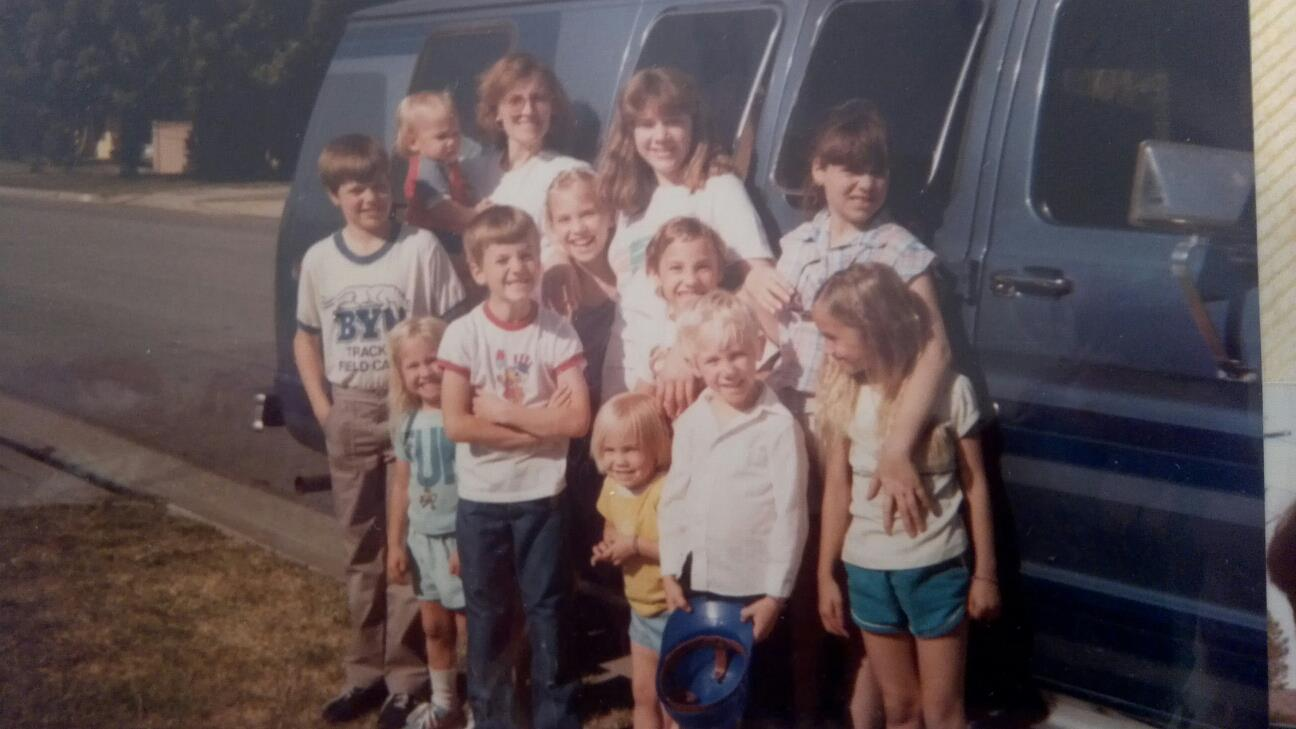
\includegraphics[width=.44\textwidth]{fig/family.jpg}
\caption{An old picture of C. Albert's family.}
\label{family}
\end{figure}

\section{Related work}

Using Poisson's equation to reconstruct and repair images is a popular because images can be transformed into vectors and completing Poisson's equation can be solved to smooth an image. From an initial analysis we have found that only recently \cite{Bertalmio} has Poisson's equation used to do image image reconstruction. The current work includes many different ways of doing image reconstruction. One field looks at taking current images that are damaged or missing parts and using gradient and Poisson to reconstruct the image. Another area looks at dragging and dropping images on top of each other then treat the resulting image as a damaged image and do the repair using Poisson.

Bertalmio et al. introduces their paper by making a goal that they want to repair damaged photos. These photos may have inpainting, meaning words written on top of the picture and remove part of the image to add the text. The authors also include photos that are damaged or missing parts of the image. Their contribution is different from other approaches as they do not require user input to define the texture of the spot being restored. They create a tool that uses partial differential equations to determine the area that is defined to be filled in. Once they fill in the area they use a smoothness function to improve the image. \cite{Bertalmio} made a major contribution by allowing restoration of images to be done automatically.

Image completion is bad in many cases because it lacks gradient of an image and thus cannot fill in missing parts of an image without having significant artifacts. To overcome this problem they introduce three steps in the process. First they introduce a gradient-patch filling to make up gradient that should be in the image. Then second they use an update strategy to gradient-patches by measure the distance between the source patch and a target in the gradient domain. Last to complete the image by using the Poisson equation on the gradient map generated by the tool.\cite{Shen} \cite{Ballester}

Image reconstruction has also been extended into restoring documents that have folds or other geometric distortions. \cite{sun} combines 3D images with restoration of documentation. The two initial challenges present themselves in using 3D images are shading, and geometric correction. The paper first solves this problem using previous work on the related subjects. Once the image has been restored to its 2D format then they solve Poisson equation and restore the image. This is work is useful for restoring documents without touching them or that may be fragile.

Mixing images is a difficult task to accomplish because the two image have different gradients. The gradients are important because it is what allows an image to seemingly mesh together. \cite{Perez} offered a solution to fixing the problem of images not being able to be place together without causing major clashing. His idea was to mix the gradients of the images together to soft of weave the two images into one another. They also made a contribution selecting only part of an image that one might want to reconstruct and then running Poisson's partial differential equation on that section. These tools that he added helped move image drag and drop along.

Drag and drop images as previously mentioned simply selected an image and dropped it onto the destination image. By doing this the destination image may contain undesired artifacts.\cite{ddp} offers a way to avoid having these artifacts by making automatic edits to the image that is being dropped into a destination image. The boundary of the image that is being dropped does not fit within the gradient of an image. This method that they use changes the boundary and makes the image fit nicer into the destination image.

\section{Poisson}

We wanted to understand all of the related work better. We wanted to understand what Poisson's equation is and how to solve it. To accomplish this task we first studied to understand how Poisson's equation works. Next we took another step and tried to understand how gradients of an image work. Then we implemented a Poisson solver to restore the image from the divergence from the gradient field. By doing this project we have learned more about Poisson's equation and how it is used to restore in image from gradient vectors.

\subsection{Poisson Equation}
\label{Poisson}
Poisson's equation is a partial differential equation that is expressed as follows:
\begin{equation} 
\ensuremath{\Delta \varphi = f}
\end{equation}
 Where \ensuremath{\Delta} is the Laplace operator. The Laplace operator is a differential operator, and \ensuremath{ \varphi(x,y) } and $ f(x,y) $ are real functions. When Poisson's equation is used in this project we it is used in 2D images. We represent the Laplacian operator as \ensuremath{\nabla^2}. This representation is to show that we are working with images in 2D space.

\begin{figure}
\centering
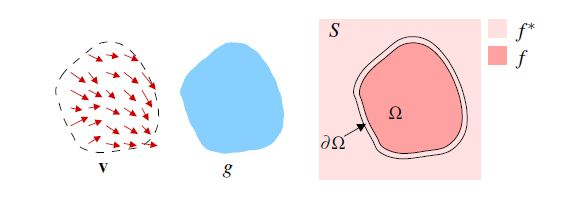
\includegraphics[width=.44\textwidth]{fig/notations.jpg}
\caption{{\bf Guided interpolation notations}. Unknown function $f$ interpolates in domain \ensuremath{\Delta} the destination function $f^*$, under guidance of vector field {\bf v}, which might be or not the gradient field of a source function $g$}
\label{notations}
\end{figure}


To further understand how this implementation works with our image editing Figure \ref{notations} taken from \cite{Perez} illustrates notations used in applying Poisson's equation to our image editing problem. S is a domain  for the function $f$ which is a closed subset of  \ensuremath{\mathbb{R}^2}. Also in the image above \ensuremath{\Omega} is a closed subset of S with the function $f^*$. {\bf v} is the vector field of image  \ensuremath{\Omega}. 

We Poisson's equation and solve the for \ensuremath{\Omega} to get an image. This can be accomplished using satisfying the associated Euler-Lagrange equation \ensuremath{\Delta f = 0} over \ensuremath{\Omega}, \ensuremath{\Delta} in our equation is represented as \ensuremath{\frac{\delta^2}{\delta x^2} + \frac{\delta^2}{\delta y^2}}. We now transform this problem into a minimization problem to solve for our image.

For the minimization problem we define it as the simplest interpolant of $f$ of $f^2$ over \ensuremath{\Omega} and represent it by the following equation:

\begin{equation}
\ensuremath{{\bf min}_f \iint_{\Omega}{|\nabla f|^2}}
\label{min}
\end{equation}

If we include the vector field {\bf v} we have a version of the the minimization problem \ref{min} but this now applies directly to the vector field {\bf v}.:

\begin{equation}
{\bf min}_f \iint_{\Omega}{|\nabla f - {\bf v}|^2}
\label{minPoisson}
\end{equation}
there problem has a unique solution with Dirichlet boundary conditions and is expressed:

\begin{equation}
\Delta f = div {\bf v} \mbox{ over \ensuremath{\Omega}}
\label{poissonEqn}
\end{equation}
We use this equation for each of the three colors in the RGB space to solve for the colored image $f$. All the results in this paper are reported with solving equation \ref{minPoisson} each color red blue and green of an image independently. In the next section we discuss how to calculate the gradient of an image.

\subsection{Gradient and Divergence}

The gradient of an image is important when solving Poisson's equation. The divergence of the vector field describe in equation \ref{poissonEqn} for our image solver is the calculation of the divergence of the gradient field. To calculate the gradient we need 1) represent the image as a scalar, 2) have an equation to calculate the gradient, 3) take care of boundary conditions, 4) calculate the divergence and 5) normalize numbers to represent results as an image.

In order to calculate a gradient we need a scalar function.
\begin{equation}
\ensuremath{f(x,y)}
\label{scalar}
\end{equation}
From this scalar function we can then take the partial derivative of $x$ and $y$ to get a gradient field. The gradient field is the rate of change in the $x$ and $y$ direction and is represented by the following equation:

\begin{equation}
\label{gradient}
\ensuremath{\nabla f = ( \frac{\delta f}{\delta x} , \frac{\delta f}{\delta y} )}
\end{equation}
To get an image gradient field we need to be able to represent the image as a scalar function. An easy way to represent the image as a scalar is to represent each pixel as a red green blue (RGB) value. The way we represent that in this paper is to have image $f$ and the variables $x$, and $y$ are the x y coordinates of the pixel in the image. The return value of this function is RGB value for each pair $(x,y)$. This is how we represent our image as a scalar function.

\begin{figure}
\centering
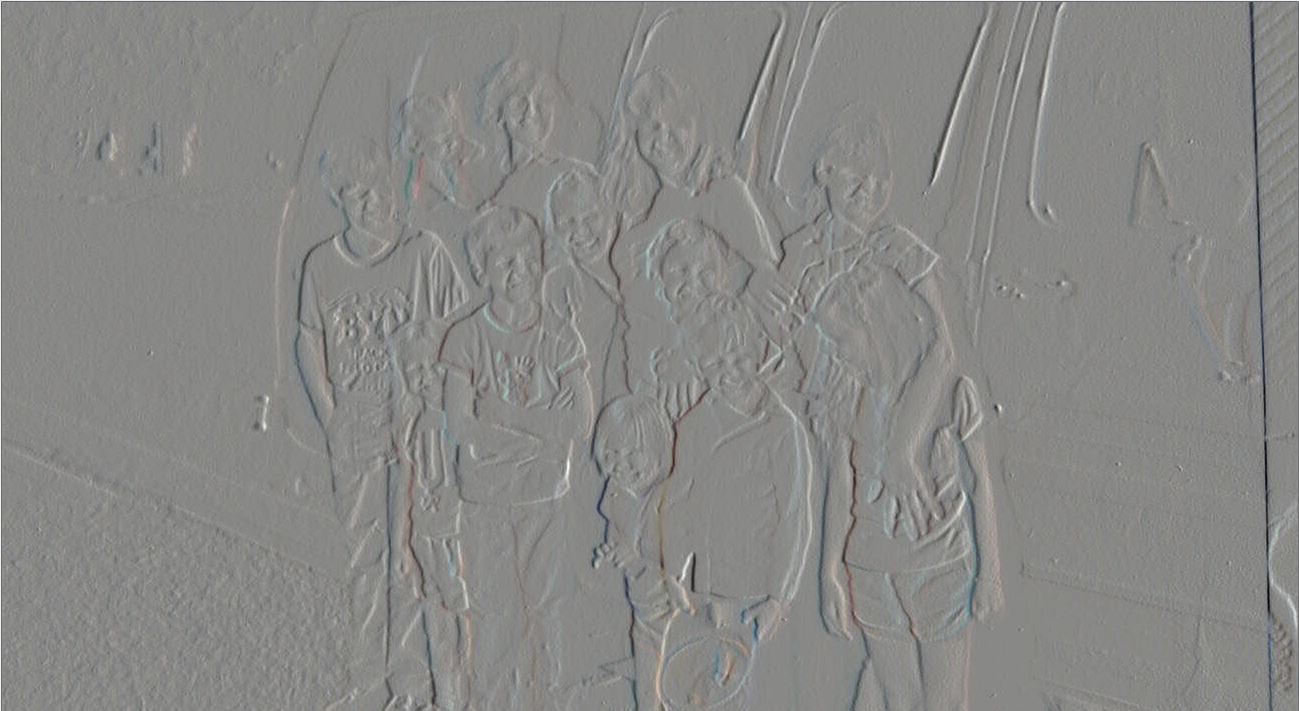
\includegraphics[width=.44\textwidth]{fig/gradientX.jpg}
\caption{\ensuremath{f_{x}}}
\label{ImageX}
\end{figure}


With the scalar function we can find the gradient field of our image. This can be calculated by taking the difference between the current and its neighbors. This is calculated with the follow equation, where \ensuremath{f_{x}} is the is the gradient in the x direction.

\begin{equation}
\ensuremath{f_{x}(i,j) = f(i)(j+1) - f(i)(j-1)}
\label{gradX}
\end{equation}

\begin{equation}
\ensuremath{f_{y}(i,j) = f(i+1)(j) - f(i-1)(j)}
\label{gradY}
\end{equation}
Using these equations we get the rate of change that happens at every pixel. 

If we were use only these equations to calculate the gradient, we end up with a picture that is one pixel smaller than the original image. One of the problems that occur when using equations \ref{gradY} and \ref{gradX} is we cannot use these equations to calculate the boundary conditions. If \ref{gradX} come to a  boundary pixel it cannot use the equation calculate the gradient because there is no $j+1$ pixel. We over come this boundary problem by duplicating every boundary pixel in both the x and y axis. Duplicating the pixels allows us to keep the original image size and still get the gradient of the image.

With the gradient field of the image we can now get the divergence which is the right hand side of the Poisson equation \ref{poissonEqn}. An example of the divergence is seen in figure \ref{div}, this image demonstrates the divergence of figures \ref{ImageY} and \ref{ImageX}. The divergence is the second derivative of equations \ref{gradY} and \ref{gradX} added together that gives us:
\begin{equation}
\label{divergence}
\ensuremath{div f = ( \frac{\delta^2 f}{\delta x^2} + \frac{\delta^2 f}{\delta y^2} )}
\end{equation}
When calculating divergence we also need to take into count the border conditions that happened with calculating the gradient. We solve the boarder problem the same way we did for gradients and duplicate each border pixel.

\begin{figure}
\centering
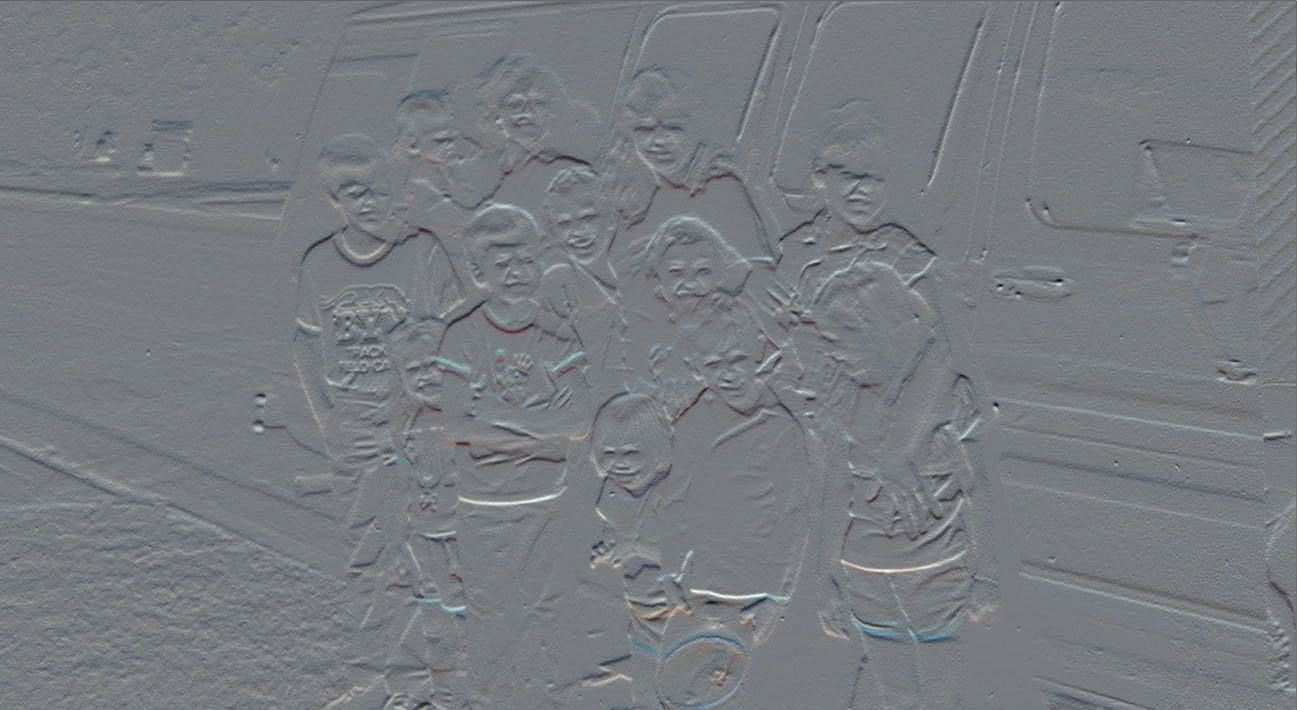
\includegraphics[width=.44\textwidth]{fig/gradientY.jpg}
\caption{\ensuremath{f_{y}}}   
\label{ImageY}
\end{figure}


\begin{figure}
\centering
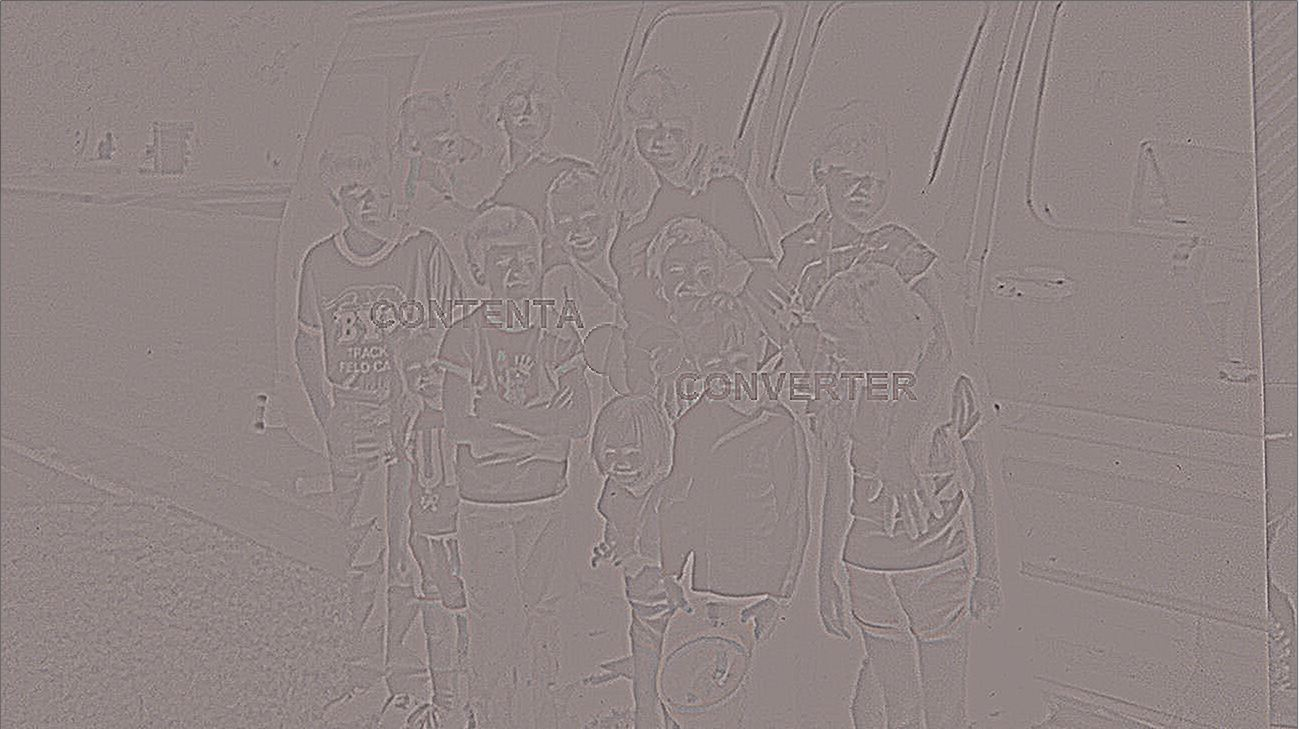
\includegraphics[width=.44\textwidth]{fig/divG.jpg}
\caption{\ensuremath{(f_{xx} + f_{yy})} Which is the divergence of \ensuremath{f_{x}} and \ensuremath{f_{y}} normalized to display in an image.}
\label{div}
\end{figure}

The calculation of the gradient gives us an array that can have the values -255 up to 255. But negative values cannot be represented in an image that has regular RGB values. In order to make the correction to display these values in a file and on this paper we normalize the array. To normalize the array we use the following function:

\begin{equation}
\label{normalize}
\ensuremath{I(x,y) = \lfloor\frac{I(x,y) - I_{min}}{I_{max} - I_{min}} \times 255 \rfloor}
\end{equation}


Normalizing the array we are able to display the gradient in the X direction with figure \ref{ImageX} and the gradient in the y direction with figure \ref{ImageY}.

\subsection{Poisson Solver}

In the Poisson's equation discussed in section \ref{Poisson} we deal with one matrix \ensuremath{\Delta} and two vectors $f$, and div {\bf v}. We know the divergence vector, but we still have two unknowns the Laplacian \ensuremath{\Delta} and $f$, which is the image we are trying to compute. We can compute $f$ in a discrete way by expressing the Laplacian and divergence as discrete filters.  But this expression is difficult to solve for large vectors so we use an iterative Jacobi Poisson solver to approximate the solution. Using the Iterative Jacobi solver we are able to regenerate an image from the divergence of that same image. 

To solve Poisson's equation \ref{poissonEqn} we need to express \ensuremath{\Delta} and the divergence as discrete filters. If we were to solve for on a single pixel grid the discretized Laplacian would look as follow:
\begin{equation}
\label{lapDes}
\Delta \rightarrow  
\left[\begin{array}{ccc}
0 & -1 & 0 \\
-1 & 4 & -1 \\
0 & -1 & 0 \end{array}\right]
\end{equation}
The divergence of the image needs to be setup to be a vector. To do this we stack the columns of the image on top of each other. The image that we need to reconstruct is also a vector of the same dimension as the divergence vector. The final representation of this equation for an image that is 4-by-4 pixels would looks like Figure \ref{poissonGrid}. This problem is now reduced to a linear system but does not scale very well as the image increases in size the size of the matrix increases by $N^2$. 

\begin{figure}%[b]
\centering
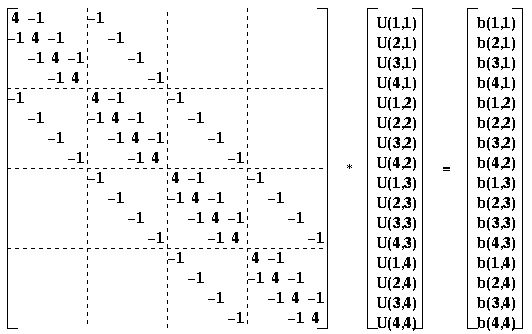
\includegraphics[width=.44\textwidth]{fig/matrix.jpg}
\caption{\ensuremath{I_{y}}}
\label{A 4-by-4 image setup as a Discrete Poisson Problem}
\end{figure}


{\bf Jacobi Method}
We use a Jacobi solver to approximate the image from the divergence, because direct solving of Poisson's equation \ref{poissonEqn} is not possible for larger images. The algorithm for the Jacobi method is as follows:

\begin{tabbing}
initialize all of f'(x,y) to 0\\
do \= \\
\> for i to n \= \\
\>\> for j to m\=\\
\>  \> f(i,j) = (f'(i-1,j)+ f'(i+1,j)+ f'(i,j-1)+ f'(i,j+1)\\
\> \>      \>       + div(i,j))/4 \\
f'(i,j) = f(i,j)\\
while (image has not converged) \\
return f(i,j)
\end{tabbing}
This algorithm needs only one input which is the divergence vector {\bf div}. It initializes the approximation of the image to zero. Then the program goes to every pixel and takes it's four neighbors and adds them and the {\bf div} of the pixel and then divides by four. This algorithm loops until the image converges or for a defined number of iterations. Our Jacobi approximation method that minimizes the differences between $\nabla f$ and $div{\bf v}$.

{\bf Applying Mask} Using a Poisson solver we can add divergences of different images together to create a transparent watermark in our resulting image. To do this we use two images, one that is our original image and another that is our watermark. Both images are the same size and the watermark has a complete white background, except for the location of the watermark. The white background allows us to locate the watermark and add together only the divergence the watermark and the picture.

\section{Artifacts}

We use the Jacobi method on a number of images and compare them to the original image. There are a few artifacts in the resulting image. The watermark functionality also can be improved. Our final images had an aveage of \result error when compared to the original image, when doing \iteration iterations.

{\bf Regenerating image} After running Jacobi method figure \ref{familyResult} is an example of the result. This image compared to the the original \ref{family} it has good coloring in the middle of the picture. One of the problems in the picture are that the boarders are white and do not have the same darker coloring of the original image. The artifacts occur due to my method of dealing with the boarder of the image, using the Jacobi method.

We tried two different methods when dealing with boarder pixels using the Jacobi method. The first way we dealt with the board pixel was to not calculate that pixel and leave it at zero. The result of that method is shown in figure \ref{familyResult}. The other method we tried was similar to calculating the gradients. When we were at a boarder pixel we duplicated the pixel and used the duplicated pixel instead of adjacent non existing pixels. The result of that image is show in figure \ref{familyBoarder}, it produced an image that was too dark. We stayed with our original method of calculating boarder pixels in the Jacobi method and left all boarder pixels at zero. 

{\bf Watermark} An example of the watermark feature of our application is show in figure \ref{mask}. The image produced by the watermark has more artifacts than only regenerating the image. We found that simply adding divergence of the watermark and the image sometimes caused the image to not have equal levels over the entire image. One of the ways that we can fix this may be to use only a small ratio of the divergence of the watermark. We did when the divergence of the watermark was small it would allow the image to produce a result much closer to that seen in when only regenerating an image.

\begin{figure}
\centering
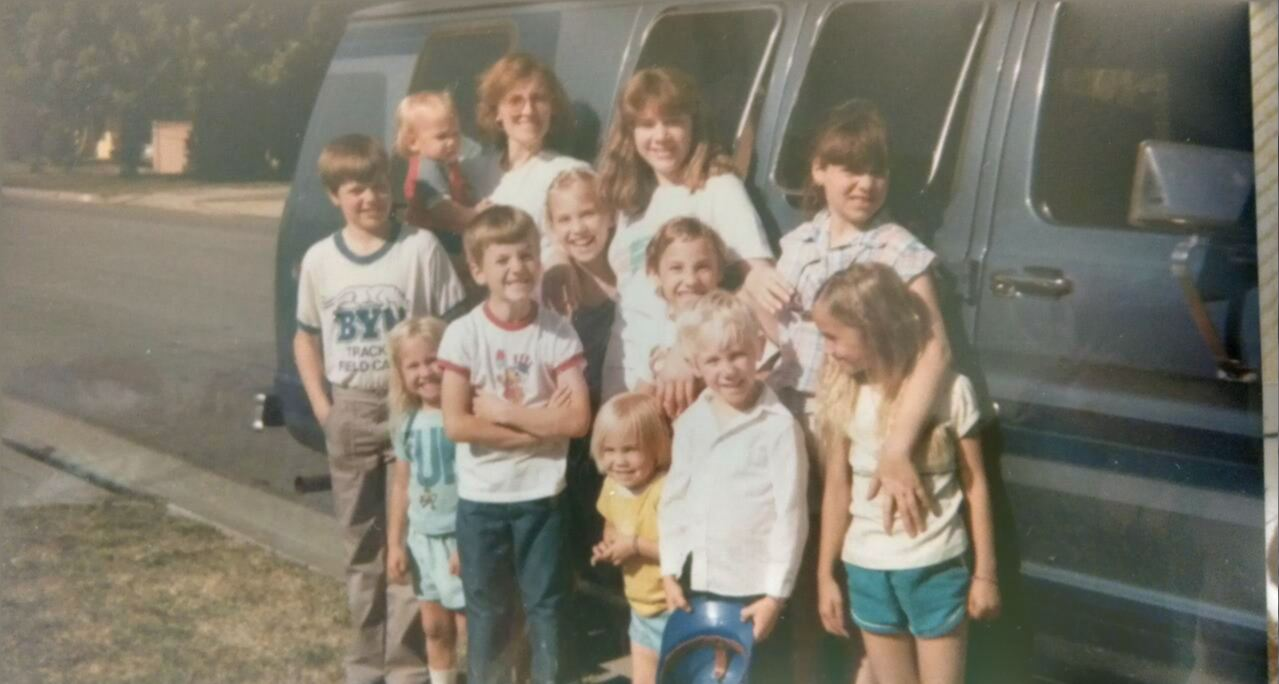
\includegraphics[width=.44\textwidth]{fig/familyResult.jpg}
\caption{An approximation using Jacobi method to solve for the original image.}
\label{familyResult}
\end{figure}


\begin{figure}
\centering
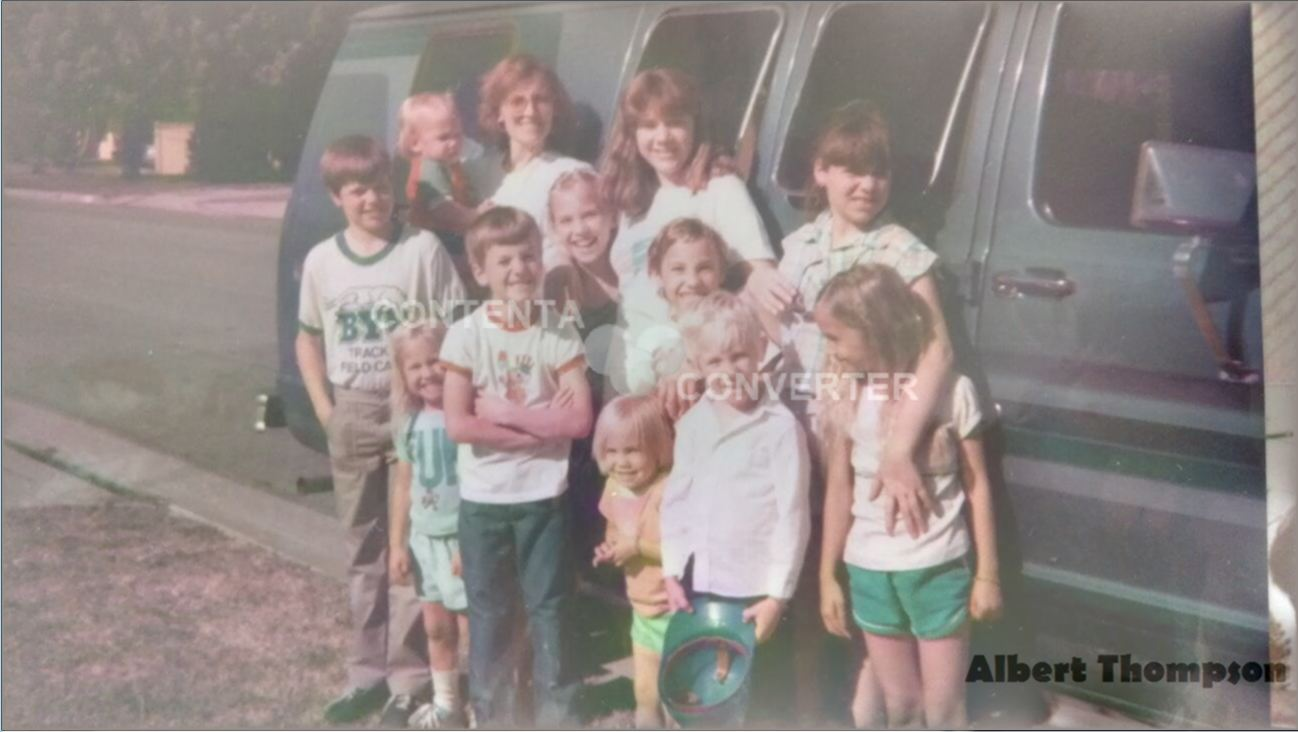
\includegraphics[width=.44\textwidth]{fig/mask.jpg}
\caption{An example of creating a watermark on an image.}
\label{mask}
\end{figure}

\section{Future Work}

Generating images using Poisson's equation allows us to do things like change gradients of images, drag and drop images as discussed in future work. We were able to produce initial results on drag and dropping images. Adding a watermark to an image is very similar to how drag and dropping discussed by \cite{ddp} works. Further work would be to add in calculations to improve the boarder of the image that is being pasted on. Also we could do more work in allowing a cut image to be transparent on the destination image. 

We also would like to explore how to estimate divergences and restore images that are missing sections. This work is discussed by \cite{Perez}. To implement this work we need to find how to make estimations of divergence that have one two or three neighbors. After we can make the estimations then we may be able to reproduce an image that is missing significant portions. 

Other work can be done on changing what Poisson solver we use. There are many different methods that can compute the linear equation (\ref{poissonEqn}) and minimize the difference in the original image and desired image. The Jacobi method works in $N^2$ space. Other methods like fast fourier transform, multigrid and conjugate gradient can be used to solve the same equations.

\section{Conclusion}

In this project we were able to make significant strides to better understanding how Poisson's equation. We learned how to calculate gradients of an image and also take in to account the boarder conditions. We also found how to solve Poisson's equation using the Jacobi method. After we did this work we were able to conduct a test with our program and see if we could return an image from our original image. In the end we were able to obtain images that looked similar to our original image.

Using the Jacobi method provided us with good experience to understand how gradients can be manipulated to produce different results in an image.  In addition to reproducing our original image we implemented a method to add a watermark to our images. Implementing our watermark method allowed us to better understand how images react when two divergences are added together. We can continue this work and implement further gradient manipulations and refine our methods of calculating boundary conditions.





\bibliographystyle{acmsiggraph}
{\small\bibliography{bibliography}}

%%%%%%%%%%%
%
% Do not change anything below this line!!!
%
%%%%%%%%%%%


% adds an empty page to documents with odd page number. This is to
% make sure that the first page of every paper starts at an odd page.
\cleardoublepage

\end{document}

% LocalWords:  CPSC Heidrich PDF cpsc tex dvi xdvi BibTeX bibtex PostScript ps
% LocalWords:  dvips Ppdf pdf pdflatex EPS PNG includegraphics
